%%% Local Variables:
%%% TeX-master: "eunchurn_park"
%%% End:
\cvevent{\printinfo{\faPlusSquare}{신세계 반포단지 구조 건전도 모니터링}}{Side project}{2022.01 -- now}{Seoul, Korea}

\begin{itemize}[label=\emoji{satellite}]
	\item DAQ 데이터 브로커 앱 개발
	      \begin{itemize}[label=\emoji{pushpin}]
		      \item 개발 기간: 2주
		      \item 개발 인원: 1명
		      \item 개발한 서비스
		            \begin{itemize}
			            \item 실시간 센서 모니터링을 위한 DAQ 브로커
			            \item NI LabVIEW 데이터 파서
			            \item 개발 스택: NI LabVIEW, TypeScript, Docker, NextJS
		            \end{itemize}
	      \end{itemize}
	\item SHM 플랫폼 개발
	      \begin{itemize}[label=\emoji{pushpin}]
		      \item 개발 기간: 1년
		      \item 개발 인원: 4명 (센서 및 장비설치 1인, 백엔드 1인, 프론트 1인, 디자이너 1인)
		      \item 개발한 서비스
		            \begin{itemize}
			            \item 실시간 센서 데이터 송수신 Worker 개발: Redis, InfluxDB, Minio
			            \item 실시간 센서 데이터 차트
			            \item 히스토리 데이터 차트: 데이터 구간별 차트 Resampling
			            \item 이벤트 리스트 및 이벤트 알림
		            \end{itemize}
		      \item 인프라 구성
		            \begin{itemize}
			            \item Bare metal 쿠버네티스 클러스터 구성: PostgreSQL, Prometheus, Grafana, NginX, Cert-manager, InfluxDB, Deployment(Web, Worker, API)
			            \item 인프라 관리: OpenLens
			            \item 배포 파이프라인: Github Action, Github container registry, ArgoCD
		            \end{itemize}
		      \item 개발 스택:
		            \begin{itemize}
			            \item Turbo Repo, TypeScript, NextJS(App router), Apollo Server, Paljs, Nexus GraphQL, MQTTjs, Redis 등
		            \end{itemize}
	      \end{itemize}
\end{itemize}
\begin{figure}[!ht]
	\begin{fullwidth}
		\parbox{0.35\textwidth}{
			\centering
			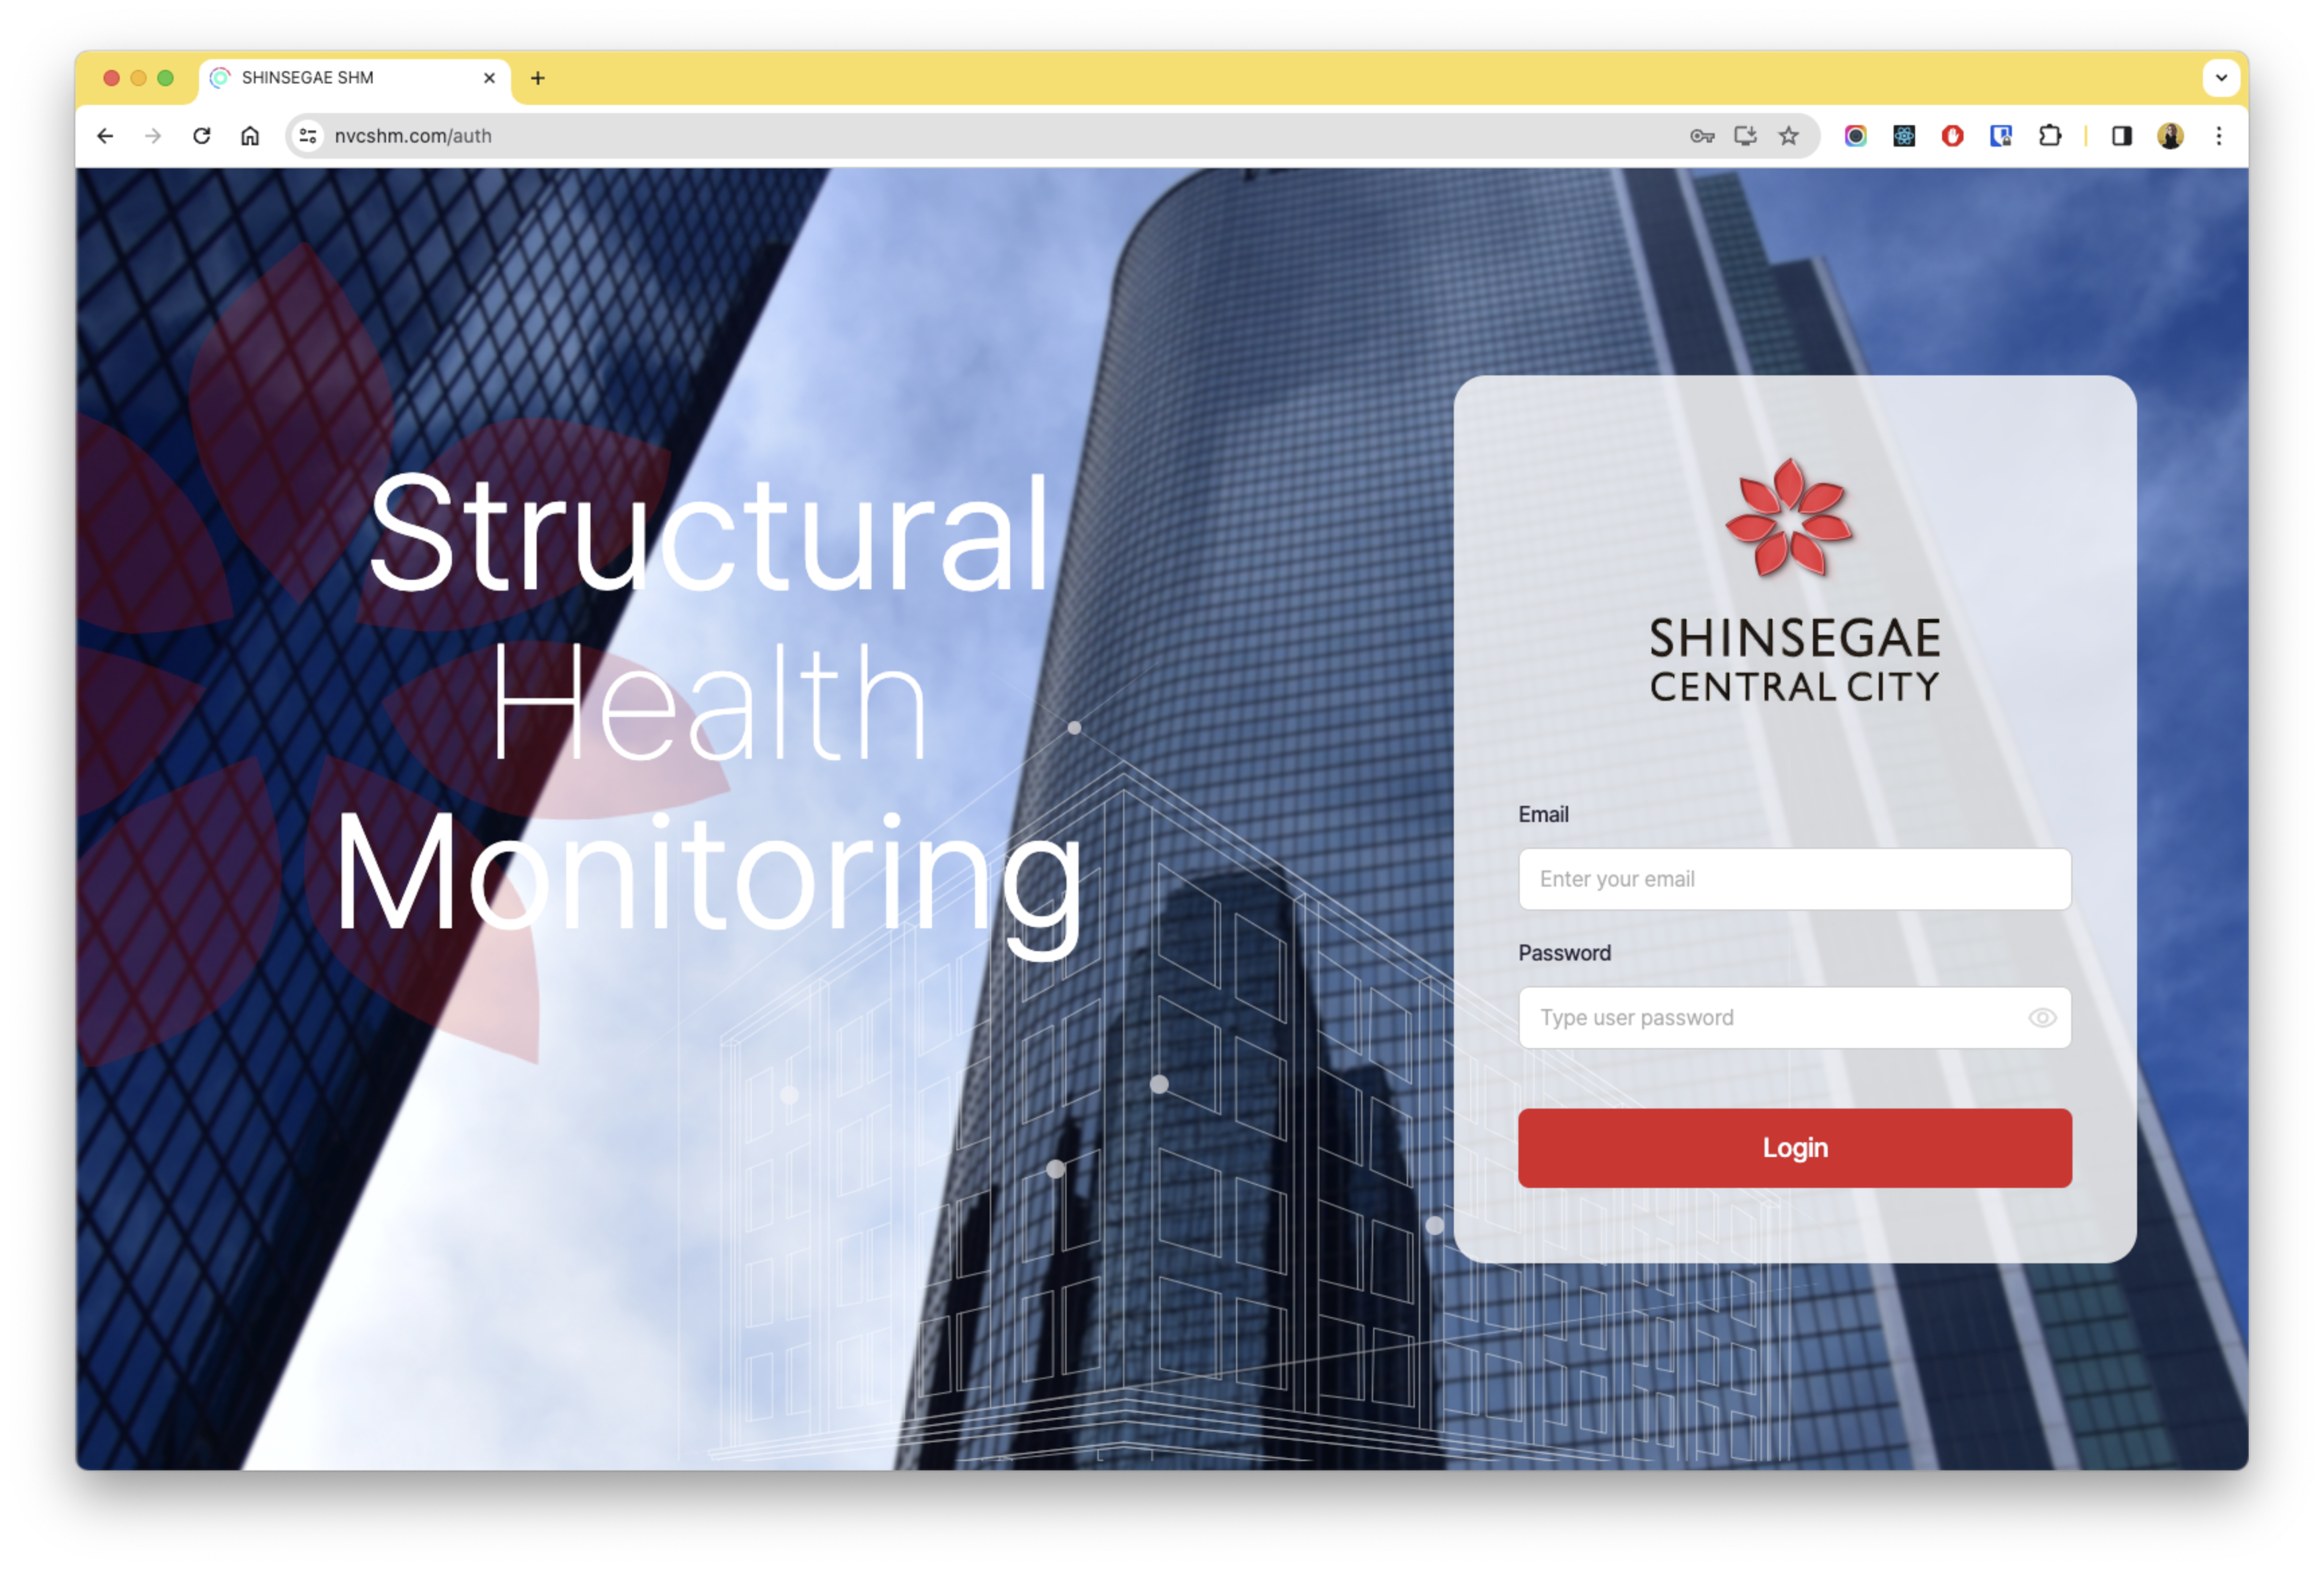
\includegraphics[width=0.35\textwidth]{images/nvcshm-auth.png}
			\caption*{Authentication}
		}\qquad
		\parbox{0.35\textwidth}{
			\centering
			\includegraphics[width=0.35\textwidth]{images/nvcshm-map.png}
			\caption*{District Map}
		}\qquad
		\parbox{0.35\textwidth}{
			\centering
			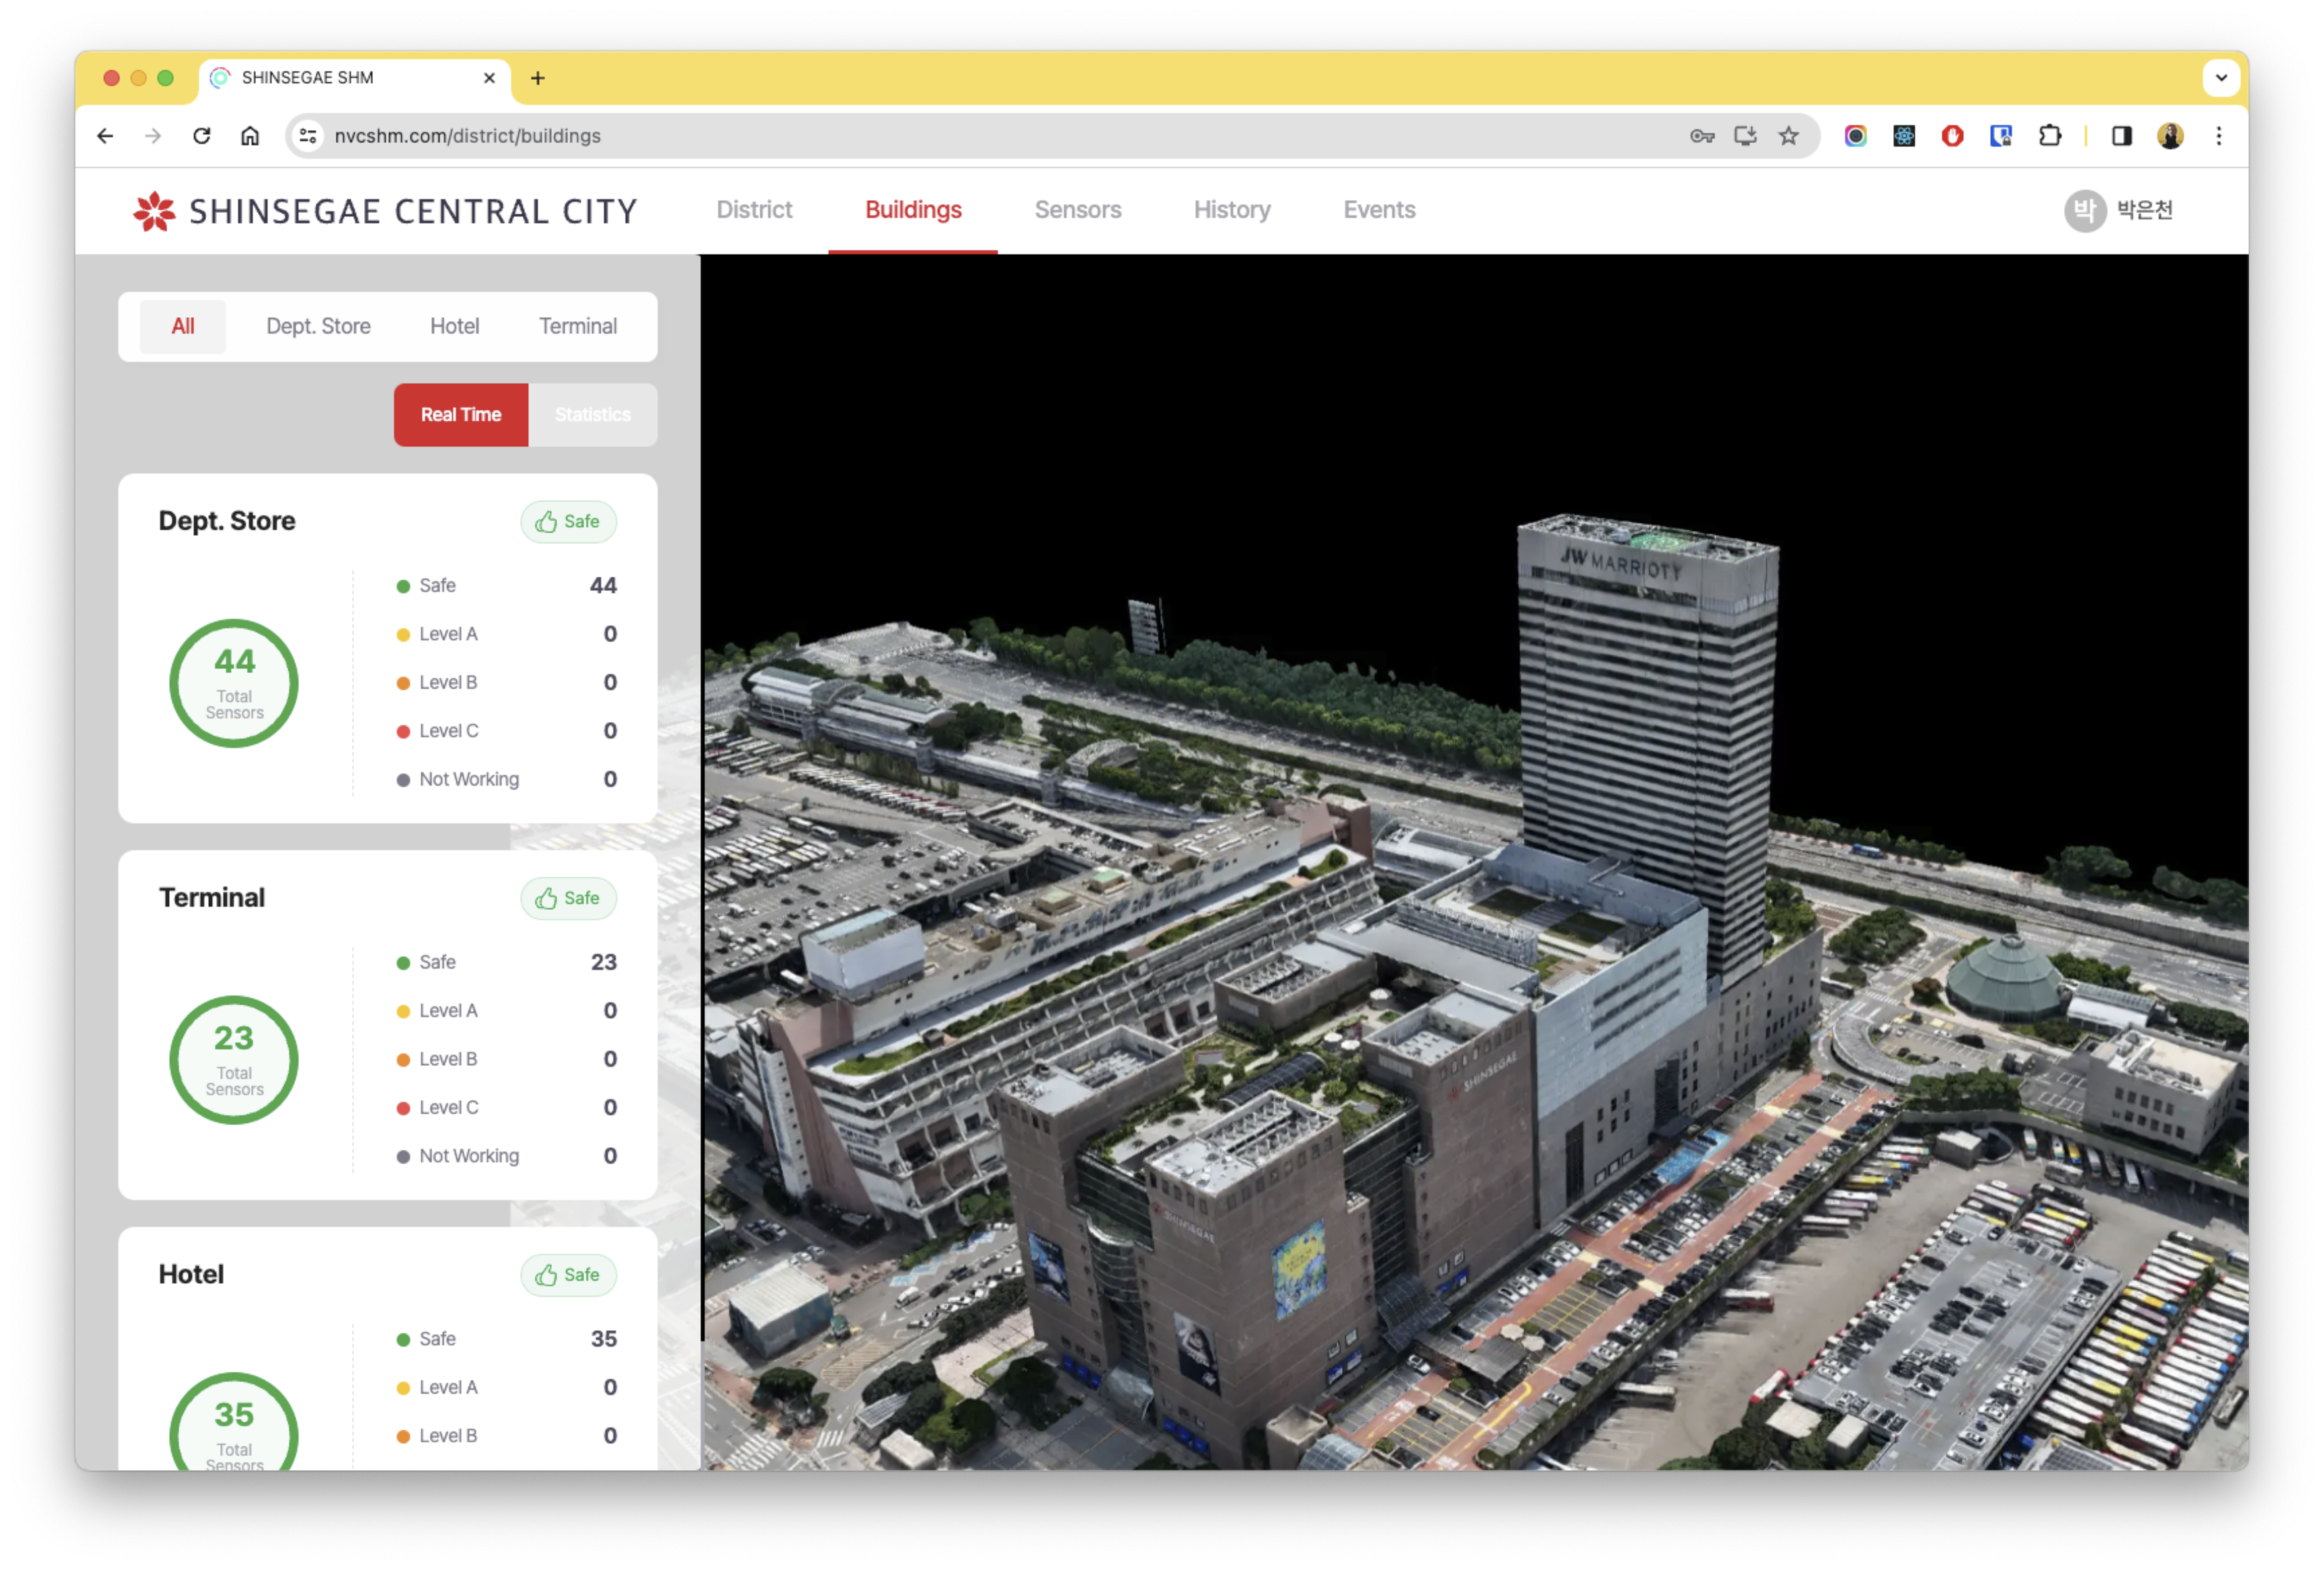
\includegraphics[width=0.35\textwidth]{images/nvcshm-building.png}
			\caption*{Building status}
		}\qquad
		\parbox{0.35\textwidth}{
			\centering
			\includegraphics[width=0.35\textwidth]{images/nvcshm-sensors.png}
			\caption*{Sensors list}
		}
		\parbox{0.35\textwidth}{
			\centering
			\includegraphics[width=0.35\textwidth]{images/nvcshm-sensor-realtime.png}
			\caption*{Sensor real-time data}
		}\qquad
		\parbox{0.35\textwidth}{
			\centering
			\includegraphics[width=0.35\textwidth]{images/nvcshm-events.png}
			\caption*{Event list}
		}\qquad
		\parbox{0.35\textwidth}{
			\centering
			\includegraphics[width=0.35\textwidth]{images/nvcshm-event-detail.png}
			\caption*{Event detail}
		}\qquad
		\parbox{0.35\textwidth}{
			\centering
			\includegraphics[width=0.35\textwidth]{images/nvcshm-history-list.png}
			\caption*{History list(sensors)}
		}
		\parbox{0.35\textwidth}{
			\centering
			\includegraphics[width=0.35\textwidth]{images/nvcshm-history-1hr.png}
			\caption*{History past 1Hr}
		}\qquad
		\parbox{0.35\textwidth}{
			\centering
			\includegraphics[width=0.35\textwidth]{images/nvcshm-history-24hr.png}
			\caption*{History past 24Hr}
		}\qquad
		\parbox{0.35\textwidth}{
			\centering
			\includegraphics[width=0.35\textwidth]{images/nvcshm-history-1w.png}
			\caption*{History past 1 Week}
		}\qquad
		\parbox{0.35\textwidth}{
			\centering
			\includegraphics[width=0.35\textwidth]{images/nvcshm-history-1m.png}
			\caption*{History past 1 Month}
		}
	\end{fullwidth}
\end{figure}